%%%%%%%%%%  TEMPLATE LAST EDITED BY PRADIPTA GHOSH on 18/01/2020 %%%%%%%%%%%%%%%%%%%%
%
%  BTP PROGRESS REPORT -- Phase-field modelling of cell crawling
%
%  COMPILE WITH pdflatex.
%
%  REQUIRED IMAGE FILES
%  --------------------
%  In the same folder as this .tex file:
%      Logo-IITD.jpg                  (supplied with the template)
%  In a subfolder called  figures/ :
%      fig_v2_shapes.pdf
%      fig_v2_transition.pdf
%      fig_v3_morph.pdf
%      fig_v3_decomp.pdf
%      fig_v4_montage.pdf
%      fig_v4_snapshots.pdf
%      fig_v4_diagnostics.pdf
%      fig_v4_area.pdf
%
%  THINGS TO FILL IN BEFORE SUBMITTING  (search for FILLME)
%  -------------------------------------------------------
%      course code, academic year and semester
%      student name(s) and entry number(s)
%      adviser name(s)
%
%%%%%%%%%%%%%%%%%%%%%%%%%%%%%%%%%%%%%%%%%%%%%%%%%%%%%%%%%%%%%%%%%%%%%%%%%%%%
\documentclass[11pt]{article}
\voffset=-2.8cm
\hoffset=-1.6cm
\textwidth=14.5cm
\textheight=24.5cm
\usepackage{amsmath}
\usepackage{amsfonts}
\usepackage{amssymb}
%\usepackage{subfig}
\usepackage{epsfig}
\usepackage{hyperref}
%\usepackage[utf8]{inputenc}
%\usepackage{mathtools}
\usepackage[caption=false]{subfig}
\usepackage{soul,xcolor}


%\vspace*{-2cm}
%%%%%%%%%%%%%%%%%%%%%%%%%%%%%%%%%%%%%%%%%%%%%%%%%%%%%%%%%%%%%%%%%%%
\begin{document}
%%%%%%%%%%%%%%%%%%%%%%%%%%%%%%%%%%%%%%%%%%%%%%%%%%%%%%%%%%%%%%%%%%%
\thispagestyle{empty}
\begin{center}
 
\includegraphics[height=3.5cm,angle=0]{Logo-IITD.jpg}\\
\textbf{Dept of Physics, IIT Delhi}
\end{center}

\vspace*{0.5cm}
\begin{center}
\textbf{Course Code : PYD411}\\      % FILLME: pick PYD411 / PYD412 / PYD414
\textbf{Academic Year : 2025 - 2026,\, Semester - I}   % FILLME
\end{center}

\vspace*{0.5cm}
\begin{center}
\textbf{\Huge{Phase-Field Modelling}}\\[0.25cm]
\textbf{\Huge{of Crawling Cells}}\\[0.45cm]
\textbf{\Large{Towards a Tractable Two-Dimensional Model}}\\
\end{center}

\vspace*{0.5cm}
\begin{center}
\textbf{\Large{Name of student 1 (Entry number)}}\\        % FILLME
%\textbf{\Large{Name of student 2 (Entry number)}}\\       % FILLME (uncomment if two students)
\end{center}

\vspace*{0.5cm}
\begin{center}
\textbf{\Large{Adviser: Prof. Firstname Middlename Lastname}}\\   % FILLME
%\textbf{\Large{\hspace*{2.1cm} Prof. Firstname Middlename Lastname}}\\
\end{center}

\vspace*{0.6cm}
\noindent
\textbf{Abstract}: Eukaryotic cells crawling on a substrate move by a combination of
actin treadmilling at the front and myosin-driven contraction at the rear. We
implement a continuum phase-field description of this process, in which a diffuse
cell field $\phi$ is coupled to a coarse-grained actin polarization $\mathbf{P}$,
and we build the model up in four controlled stages so that the role of each
physical ingredient can be isolated. The baseline model, with the fluid velocity
set to zero, translates a cell rigidly but cannot deform it and loses $4.5\%$ of
its area. Confining treadmilling to a thin layer near the substrate in a
vertical slice produces a thin leading protrusion and steady crawling, with a
protrusion transition as the treadmilling rate is increased. The complete model
in the plane, including an incompressible Stokes flow, active and elastic
stresses and boundary anchoring, reproduces the non-motile actin aster and the
lamellipodial fan of Tjhung \textit{et al.} Isolating the ingredients shows that
in this geometry the cell shape is set almost entirely by anchoring-induced splay
of $\mathbf{P}$, the hydrodynamic flow contributing about $2\%$. Guided by this,
we replace the elliptic Stokes solve by its friction-dominated limit, in which
the force balance becomes local algebra. The resulting model is roughly five
times faster, agrees with the full calculation to $0.2\%$ where the two coincide,
conserves cell volume rather than projected area, and is local in structure,
which is the property required to extend the work to many interacting cells.

\vspace*{1.0cm}
\begin{flushleft}
Signature of the student: ................
\end{flushleft}

\vspace*{-1.2cm}

\begin{flushright}
Signature of the adviser: ................
\end{flushright}

%%%%%%%%%%%%%%%%%%%%%%%%%%%%%%%%%%%%%%%%%%%%%%%%%%%%%%%%%%%%%%%%%%%%%%%%%%
\newpage
\thispagestyle{empty}
.
\newpage
% DO NOT TOUCH THIS PART. THIS WILL MAKE SURE THAT
%THE SECOND PAGE, AFTER THE TITLE PAGE SHOULD REMAIN EMPTY
\clearpage
\setcounter{page}{1}
%%%%%%%%%%%%%%%%%%%%%%%%%%%%%%%%%%%%%%%%%%%%%%%%%%%%%%%%%%%%
%%%%%%%%%%%%%%%%%%%%%%%%%%%%%%%%%%%%%%%%%%%%%%%%%%%%%%%%%%%%
\section{Introduction and Motivation}
\label{sec:intro}

\noindent
The ability of a eukaryotic cell to crawl over a solid surface underlies wound
healing, immune response and the metastatic spread of cancer. The mechanical
picture, established by decades of cell biology, involves three ingredients
\cite{Bray:2000}. Actin filaments polymerise at their leading end and
depolymerise at the trailing end, so that a polarised actin network
``treadmills'' and pushes the front of the cell forward. Myosin motors walking
along those filaments generate a contractile stress that helps retract the rear.
Finally, focal adhesions couple the actomyosin network mechanically to the
substrate, and the strength of that coupling controls how efficiently internal
force is converted into motion.

A natural question is how much of this behaviour is genuinely
\textit{mechanical}, as opposed to being orchestrated moment-to-moment by
biochemical signalling. The experimental evidence that a large part of it is
mechanical is striking: fragments of keratocytes that have been cut off from the
cell body, and which therefore lack the nucleus and most of the regulatory
machinery, nevertheless polarise spontaneously and crawl in a persistent and
directed way \cite{Verkhovsky:1999}. The shapes such cells adopt are also
reproducible enough to be predicted from a small number of mechanical parameters
\cite{Keren:2008}, and experiments in which substrate adhesion is varied show
that adhesion strength alone can switch a cell between distinct shape and
motility regimes \cite{Barnhart:2011}. Taken together, these results motivate the
construction of \textit{minimal physical models}: models built only from
mechanics and thermodynamics, with as few parameters as possible, whose purpose
is to identify which physical ingredients are actually necessary to reproduce an
observed behaviour.

The specific model we build on is that of Tjhung, Tiribocchi, Marenduzzo and
Cates \cite{Tjhung:2015}, who describe a crawling cell as a droplet of active
polar fluid resting on a wall. The cell material is represented by a scalar
concentration field, the actin orientation by a polarization vector field, and
the cytoplasm by an incompressible fluid whose flow is computed from a force
balance including an active stress. That work grew out of an earlier study
showing that a contractile active droplet can move spontaneously in bulk fluid,
by breaking the symmetry of its own polarization field \cite{Tjhung:2012}. In
three dimensions the model of Ref.~\cite{Tjhung:2015} produces a remarkable
variety of shapes that resemble real cells, including the flat fan-shaped
lamellipodium of a motile keratocyte, a finger-like pseudopod, and a
non-motile ``fried egg''.

A quite different modelling tradition treats the substrate coupling in
microscopic detail instead. Leoni and Sens \cite{Leoni:2017} model a cell as a
set of oscillating force dipoles bound to the substrate through stochastic
linkers, and show that directed crawling requires those linkers to be
\textit{mechanosensitive}: the bond lifetime must depend on load, so that the
effective drag differs between the protrusion and the retraction phase of a
cycle. Averaged over many binding and unbinding events, their treatment reduces
to an effective friction force on the cell, which is precisely how substrate
adhesion enters depth-averaged continuum models of the kind used by Ziebert and
Aranson \cite{Ziebert:2013}. That connection is what we exploit in
Sec.~\ref{sec:v4}.

The eventual goal of this project is to simulate \textit{many} crawling cells and
their mutual interaction. This changes what counts as a good model. The
formulation of Ref.~\cite{Tjhung:2015} requires the solution of an elliptic
(Stokes) problem at every time step, in which the velocity at each point depends
on the forces everywhere; such a global coupling is expensive for one cell and
becomes prohibitive for many. The work reported here therefore has two parallel
aims: first, to implement and verify the full model so that we understand what it
does and which of its ingredients matter; and second, to use that understanding
to construct a cheaper model whose accuracy we can quantify against the full one.
We proceed in four stages, summarised in table~\ref{tab:versions}.

%%%%%%%%%%%%%%%%%%%%%%%%%%%%%%%%%%%%%%%%%%%%%%%%%%%%%%%%%%%%
\begin{table} [ht!]
\begin{center}
\begin{tabular}{ |c|c|c|c| }
 \hline
 Version & Geometry & Force balance & Cell area \\
 \hline
 1 & plane, free space & $\mathbf{v}=0$ & drifts by $4.5\%$ \\
 \hline
 2 & slice with a wall & screened in $z$ & fixed exactly \\
 \hline
 3 & plane, friction & incompressible Stokes & fixed exactly \\
 \hline
 4 & plane, friction & friction dominated & free, soft \\
 \hline
\end{tabular}
\end{center}
\caption{The four stages of the model. Version 1 is the starting point, in which
the fluid velocity is switched off. Versions 2 and 3 are complementary rather
than sequential: the protrusion of Ref.~\cite{Tjhung:2015} is a near-substrate
structure and requires the vertical slice, whereas its cell shapes are top-view
shapes and require the plane. Version 4 is the tractable model that the
multi-cell work will be built on.}
\label{tab:versions}
\end{table}
%%%%%%%%%%%%%%%%%%%%%%%%%%%%%%%%%%%%%%%%%%%%%%%%%%%%%%%%%%%%

%%%%%%%%%%%%%%%%%%%%%%%%%%%%%%%%%%%%%%%%%%%%%%%%%%%%%%%%%%%%
%%%%%%%%%%%%%%%%%%%%%%%%%%%%%%%%%%%%%%%%%%%%%%%%%%%%%%%%%%%%
\section{Computational Setup}
\label{sec:model}

\noindent
In this section \ref{sec:model} we set out the free energy, the equations of
motion and the numerical methods. Throughout, $\phi(\mathbf{r},t)$ is a diffuse
field equal to $1$ inside the cell and $0$ outside, $\mathbf{P}(\mathbf{r},t)$ is
the coarse-grained actin polarization, and $\mathbf{v}(\mathbf{r},t)$ is the
velocity of the cytoplasm.

%%%%%%%%%%%%%%%%%%%%%%%%%%%%%%%%%%%%%%%%%%%%%%%%%%
\noindent
\subsection{Free energy}
\label{subsec:freeenergy}

Following Ref.~\cite{Tjhung:2015} the equilibrium physics is generated by
\begin{eqnarray}\label{eq:F}
F[\phi,\mathbf{P}]=\int d^2r\,\Big\{
a\,\phi^{2}(\phi-1)^{2}
&+&\frac{\varepsilon^{2}}{2}|\nabla\phi|^{2}
-\frac{\alpha}{2}\left(2\phi-1\right)|\mathbf{P}|^{2}\nonumber\\
&+&\frac{\alpha}{4}|\mathbf{P}|^{4}
+\frac{\kappa}{2}\left(\nabla\mathbf{P}\right)^{2}
+\beta\,\mathbf{P}\cdot\nabla\phi\Big\}.
\end{eqnarray}
The first term is a double well that stabilises the cell interior
($\phi=1$) and the exterior ($\phi=0$), and the second penalises interface area,
so that together they generate an interfacial tension and a diffuse interface of
width $\varepsilon$. The third and fourth terms drive an isotropic-to-polar
transition \textit{inside} the cell only: minimising them gives
$|\mathbf{P}|^{2}=2\phi-1$, so that $|\mathbf{P}|\to1$ deep inside the cell and
$\mathbf{P}\to0$ outside, smoothly across the interface. The fifth term is the
Frank elastic energy of a polar liquid crystal in the one-constant approximation
\cite{deGennes:1993}, which makes neighbouring regions of the actin network want
to point the same way. The last term is the \textit{anchoring}: for $\beta>0$ the
polarization prefers to point outward, normal to the cell boundary, and for
$\beta<0$ inward. As we shall see in Sec.~\ref{sec:results}, $\beta$ turns out to
be the single most important shape parameter.

Differentiating eq.(\ref{eq:F}) gives the chemical potential of the cell field
and the molecular field conjugate to the polarization,
\begin{eqnarray}\label{eq:mu_h}
\mu_\phi\equiv\frac{\delta F}{\delta\phi}&=&2a\,\phi(\phi-1)(2\phi-1)
-\varepsilon^{2}\nabla^{2}\phi-\alpha|\mathbf{P}|^{2}
-\beta\,\nabla\cdot\mathbf{P},\nonumber\\
\mathbf{h}\equiv\frac{\delta F}{\delta\mathbf{P}}
&=&\left[-\alpha(2\phi-1)+\alpha|\mathbf{P}|^{2}\right]\mathbf{P}
-\kappa\nabla^{2}\mathbf{P}+\beta\nabla\phi.
\end{eqnarray}
Note that the two fields are coupled thermodynamically in both directions,
through the $-\alpha|\mathbf{P}|^{2}$ and $-\beta\nabla\cdot\mathbf{P}$ terms in
$\mu_\phi$ and the $\beta\nabla\phi$ term in $\mathbf{h}$.

%%%%%%%%%%%%%%%%%%%%%%%%%%%%%%%%%%%%%%%%%%%%%%%%%%
\noindent
\subsection{Equations of motion}
\label{subsec:eom}

Cell material is transported by the sum of the fluid velocity and the
treadmilling velocity, $\mathbf{u}=\mathbf{v}+w_{0}\mathbf{P}$, where $w_{0}$ is
the speed at which a filament self-propels along its own tangent relative to the
fluid, and is therefore proportional to the rate of actin polymerisation. The
cell field and the polarization then obey
\begin{eqnarray}\label{eq:eom}
\frac{\partial\phi}{\partial t}+\nabla\cdot\left(\phi\,\mathbf{u}\right)
&=&-M\left[\mu_\phi-\Lambda\,g(\phi)\right],\nonumber\\
\frac{\partial\mathbf{P}}{\partial t}
+\left(\mathbf{u}\cdot\nabla\right)\mathbf{P}
&=&-\mathbf{\Omega}\cdot\mathbf{P}+\chi\,\mathbf{D}\cdot\mathbf{P}
-\frac{1}{\Gamma}\mathbf{h},
\end{eqnarray}
where $\mathbf{D}$ and $\mathbf{\Omega}$ are the symmetric and antisymmetric
parts of the velocity gradient tensor $\partial_\alpha v_\beta$, so that the
first term on the right rotates $\mathbf{P}$ with the local vorticity and the
second aligns it with the straining direction of the flow. $\Gamma$ is a
rotational viscosity. The term involving $\Lambda$ enforces the volume
constraint and is discussed in Sec.~\ref{subsec:volume}.

The cell is at Reynolds number of order $10^{-5}$, so inertia is negligible and
the force balance is the Stokes limit of the Navier--Stokes equation. Because we
work in a top view, the substrate is not part of the computational domain, so the
no-slip wall of Ref.~\cite{Tjhung:2015} is represented by a depth-averaged
friction $-\xi\mathbf{v}$. This is exactly the description of adhesion that
Ref.~\cite{Leoni:2017} arrives at by averaging over the stochastic binding and
unbinding of substrate linkers, and $\xi$ is inversely related to the density of
focal adhesions. The force balance reads
\begin{equation}\label{eq:stokes}
0=-\nabla p+\eta\nabla^{2}\mathbf{v}-\xi\mathbf{v}+\mathbf{f},
\qquad \nabla\cdot\mathbf{v}=0,
\end{equation}
with the body force
\begin{equation}\label{eq:force}
f_\alpha=\partial_\beta\left(\sigma^{act}_{\alpha\beta}
+\sigma^{el}_{\alpha\beta}\right)-\phi\,\partial_\alpha\mu_\phi.
\end{equation}
Here the active stress and the elastic stress are
\begin{eqnarray}\label{eq:stresses}
\sigma^{act}_{\alpha\beta}&=&-\zeta\,\phi\,P_\alpha P_\beta,\nonumber\\
\sigma^{el}_{\alpha\beta}&=&\frac{1}{2}\left(P_\alpha h_\beta-P_\beta h_\alpha\right)
-\frac{\chi}{2}\left(P_\alpha h_\beta+P_\beta h_\alpha\right)
-\kappa\,\partial_\alpha P_\gamma\,\partial_\beta P_\gamma,
\end{eqnarray}
and the last term of eq.(\ref{eq:force}) is the capillary force, which is the
interfacial stress of Ref.~\cite{Tjhung:2015} written in potential form; the two
differ only by a gradient, which the pressure absorbs. The activity parameter
$\zeta$ is negative for a contractile material, which is the actomyosin case: for
$\mathbf{P}$ along $\hat{x}$ one has $\sigma^{act}_{xx}=|\zeta|\phi$, and the
resulting force $|\zeta|\partial_x\phi$ points inward at the front and forward at
the rear, i.e.\ it squeezes the cell along its polarization axis.

%%%%%%%%%%%%%%%%%%%%%%%%%%%%%%%%%%%%%%%%%%%%%%%%%%
\noindent
\subsection{Conserving volume rather than area}
\label{subsec:volume}

The relaxational term $-M\mu_\phi$ in eq.(\ref{eq:eom}) restores a sharp
interface and drives motion by curvature, which is the interfacial tension we
need, but on its own it does not conserve $\int\phi\,dA$. Ref.~\cite{Tjhung:2015}
uses instead a Cahn--Hilliard form $\nabla\cdot(M\nabla\mu_\phi)$, which
conserves it identically but is fourth order in space and would require
$dt\sim dx^{4}$ in an explicit scheme.

We therefore keep the second-order operator and subtract a spatially uniform
Lagrange multiplier, weighted by $g(\phi)=\phi(1-\phi)$ so that the correction
acts only where the interface is. Two choices of $\Lambda$ are used. The
\textit{rigid} choice
\begin{equation}\label{eq:rigid}
\Lambda=\frac{\int\mu_\phi\,dA}{\int g\,dA}
\end{equation}
makes the bracket in eq.(\ref{eq:eom}) integrate to zero, so that
$\frac{d}{dt}\int\phi\,dA=0$ exactly rather than approximately; this is the
conservative Allen--Cahn equation of Rubinstein and Sternberg
\cite{Rubinstein:1992}, and it is what Versions 2 and 3 use.

Rigid area is, however, the wrong constraint for a top-view model of a real cell.
A crawling cell is a thin sheet of roughly constant \textit{volume}
\begin{equation}\label{eq:volume}
V_{0}\simeq h(t)\,A(t),
\end{equation}
where $A$ is the projected area we see from above and $h$ is the thickness we do
not. Spreading is therefore permitted, provided it is paid for by thinning, and
pinning $A$ forbids it altogether. Version 4 accordingly replaces
eq.(\ref{eq:rigid}) by a \textit{soft} restoring force
\begin{equation}\label{eq:soft}
\Lambda=-k_{A}\left(\frac{A}{A_{0}}-1\right),
\qquad A=\int\phi\,dA,
\end{equation}
in which the stiffness $k_{A}$ represents the energetic cost of thinning, due for
instance to cortical tension. It interpolates between the two extremes:
$k_{A}\to\infty$ recovers rigid area, and $k_{A}=0$ removes the constraint
altogether. Since it is $V_{0}$ that is conserved, we report the implied
thickness $h=V_{0}/A$ alongside the area.

%%%%%%%%%%%%%%%%%%%%%%%%%%%%%%%%%%%%%%%%%%%%%%%%%%
\noindent
\subsection{Numerical methods}
\label{subsec:numerics}

All fields are discretised on a uniform periodic grid with central-difference
stencils and advanced with an explicit Euler step. Four points deserve comment.

\textbf{Conservative advection.} The transport term is evaluated in flux form on
cell faces, $F^{x}_{i+1/2,j}=\frac{1}{2}(\phi_{i,j}+\phi_{i+1,j})\cdot
\frac{1}{2}(u^{x}_{i,j}+u^{x}_{i+1,j})$, so that whatever leaves one cell enters
its neighbour and the sum over the grid telescopes. Transport therefore moves
material rather than creating it, and the only term that can change the area is
the relaxation, deliberately. Version 1 instead used the non-conservative form
$\mathbf{u}\cdot\nabla\phi$ together with a clipping of $\phi$ to $[0,1]$, which
is the origin of its area drift.

\textbf{Spectral Stokes solve (Version 3).} Because the domain is periodic,
eq.(\ref{eq:stokes}) can be solved exactly in Fourier space. Contracting the
transformed equation with $k_\alpha$ and using
$\mathbf{k}\cdot\hat{\mathbf{v}}=0$ eliminates the pressure at once and leaves
\begin{equation}\label{eq:leray}
\hat{\mathbf{v}}(\mathbf{k})=\frac{1}{\xi+\eta k^{2}}
\left(\hat{\mathbf{f}}-\hat{\mathbf{k}}\,
(\hat{\mathbf{k}}\cdot\hat{\mathbf{f}})\right),
\end{equation}
a transverse (Leray) projection followed by a division. This costs one pair of
fast Fourier transforms per step, requires no iteration, and imposes no
time-step restriction from the viscous term. Note that the friction $\xi$ is what
makes the $\mathbf{k}=0$ mode well defined.

\textbf{Time step and re-centring.} With every operator second order, the binding
stability constraint is interface diffusion, $dt<dx^{2}/(4M\varepsilon^{2})$. The
cell is kept in the middle of the periodic box by rolling all arrays by a whole
number of grid cells, which is exact, conserves mass to machine precision and
introduces no interpolation error; the accumulated shifts recover the laboratory
trajectory. The box must be large enough that the cell never wraps onto itself,
and the code warns if $\phi>1/2$ reaches within a few cells of the edge.

\textbf{Diagnostics.} Besides the centre of mass and speed, we monitor the aspect
ratio from the eigenvalues of the second-moment tensor of $\phi$, the circularity
$4\pi A/\mathcal{P}^{2}$ with $\mathcal{P}=\int|\nabla\phi|dA$, the polarization
order $|\langle\mathbf{P}\rangle|$, which is close to $1$ for a uniformly
polarised cell and $0$ for an aster, the maximum flow speed, and the relative
volume error, which serves as a regression test on the conservative advection.

%%%%%%%%%%%%%%%%%%%%%%%%%%%%%%%%%%%%%%%%%%%%%%%%%%
%%%%%%%%%%%%%%%%%%%%%%%%%%%%%%%%%%%%%%%%%%%%%%%%%%
\section{Results and discussion}
\label{sec:results}

\subsection{Version 1: the baseline, and what it cannot do}
\label{sec:v1}

Version 1 solves eq.(\ref{eq:eom}) with $\mathbf{v}=0$, $\zeta=0$, $\beta=0$ and
no volume constraint, starting from a disc with $\mathbf{P}\approx(1,0)$. It
establishes the feedback loop $\mathbf{P}\rightarrow w_{0}\mathbf{P}\rightarrow$
transport $\rightarrow$ motion, and the cell does move: over $5000$ steps the
centre of mass advances linearly. Two limitations are, however, decisive.

First, the cell cannot change shape. Its aspect ratio stays between $1.00$ and
$1.01$ for the whole run, and $|\langle\mathbf{P}\rangle|$ and
$\langle|\mathbf{P}|\rangle$ lie exactly on top of each other, showing that
$\mathbf{P}$ remains perfectly uniform and never splays. This is not a numerical
failing but a structural one: if $\mathbf{P}$ is uniform then
$\mathbf{u}=w_{0}\mathbf{P}$ is uniform, and a uniform velocity can only
translate the cell. Second, the effective area falls monotonically by about
$4.5\%$, for the reason given in Sec.~\ref{subsec:numerics}. The measured speed,
$0.42$ to $0.47$, is also well below $w_{0}\langle|\mathbf{P}|\rangle\approx0.85$,
a further consequence of the non-conservative advection. Versions 2 to 4 remove
both problems.

\subsection{Version 2: a protrusion at the substrate}
\label{sec:v2}

The thin lamellipodial protrusion of Fig.~1 of Ref.~\cite{Tjhung:2015} is a
\textit{near-substrate} structure, so we study it in a vertical $(y,z)$ slice
with a wall at $z=0$. The essential ingredient is that treadmilling is confined
to a layer of thickness $\lambda$ next to the substrate,
\begin{equation}\label{eq:wz}
w(z)=\frac{w_{0}}{2}\left[1-\tanh\left(\frac{z-\lambda}{w_\tau}\right)\right].
\end{equation}
Material within $\lambda$ of the wall is pushed forward hard while material above
it is not, so the near-wall layer runs out ahead of the cell body and interfacial
tension pulls it back; the steady state of that competition \textit{is} the
protrusion, and $\lambda$ sets its thickness. With the spatially uniform $w_{0}$
of Version 1 no such gradient exists. Wall conditions are imposed with a
ghost-cell parity trick: an even mirror gives neutral wetting for $\phi$ and
leaves $P_y$ free, while an odd mirror pins $P_z=0$, which is how the
polarization becomes anchored parallel to the substrate.

Rather than solve for the flow, Version 2 uses the thin-film (Brinkman) closure
$\left(1-\ell_v^{2}\partial_z^{2}\right)\mathbf{u}=w(z)\mathbf{P}$, one
tridiagonal solve per step, with $\ell_v=\sqrt{\eta/\xi}$ a viscous screening
length. Some such coupling is necessary: with none at all, only the driven layer
moves, the cell body lags behind and the droplet shears into a flat slab, leaving
nothing for a protrusion to protrude from.

Figure~\ref{fig:v2shapes} shows two cells differing only in $w_{0}$. The slow one
remains close to a hemispherical cap and creeps along; the fast one keeps a
rounded rear but draws its near-wall material into a thin leading layer whose tip
thickness is set by $\lambda$. Both conserve volume to machine precision, with a
relative error at the $10^{-16}$ level, against the $4.5\%$ loss of Version 1.
Figure~\ref{fig:v2transition} sweeps $w_{0}$: the steady contact length is nearly
flat while $w_{0}\lesssim0.8$ and then turns sharply upward, which is the
crossover Ref.~\cite{Tjhung:2015} identifies at a critical treadmilling rate
$w_c$. The location is understood: a protrusion of thickness $h$ is pulled back
by interfacial tension at a rate $\sim M\varepsilon^{2}/h$, so a thin layer can
only be sustained once the active push exceeds roughly
$M\varepsilon^{2}/\lambda\approx0.75$ for these parameters. Our crossover is
smooth rather than discontinuous; in Ref.~\cite{Tjhung:2015} it sharpens only once
the substrate slip parameter is turned on, and slip lives in the hydrodynamic
boundary condition, which this closure does not have.

%%%%%%%%%%%%%%%%%%%%%%%%%%%%%%%%%%%%%%%%%%%%%%%%%%%%%%%%%%%%
\begin{figure}[ht!]
\centering
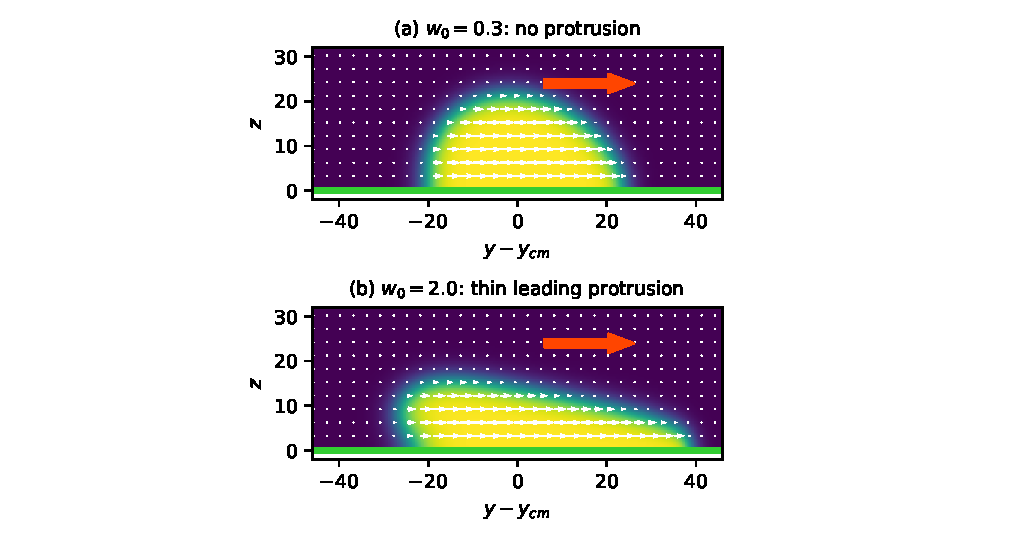
\includegraphics[width=14cm]{figures/fig_v2_shapes.pdf}
\caption{{Version 2, steady crawling shapes in a vertical slice with a no-slip
wall (green) at $z=0$; the cell moves to the right. White arrows show the actin
polarization $\mathbf{P}$. The two runs differ \textit{only} in the treadmilling
rate. (a) At $w_{0}=0.3$ the cell stays close to a hemispherical cap and creeps
along, with contact length $44.0$ and speed $0.050$. (b) At $w_{0}=2.0$ it keeps a
rounded rear but extends a thin leading protrusion, with contact length $63.0$
and speed $0.432$. The relative volume error is at the $10^{-16}$ level in both
cases.}}
\label{fig:v2shapes}
\end{figure}
%%%%%%%%%%%%%%%%%%%%%%%%%%%%%%%%%%%%%%%%%%%%%%%%%%%%%%%%%%%%

%%%%%%%%%%%%%%%%%%%%%%%%%%%%%%%%%%%%%%%%%%%%%%%%%%%%%%%%%%%%
\begin{figure}[ht!]
\centering
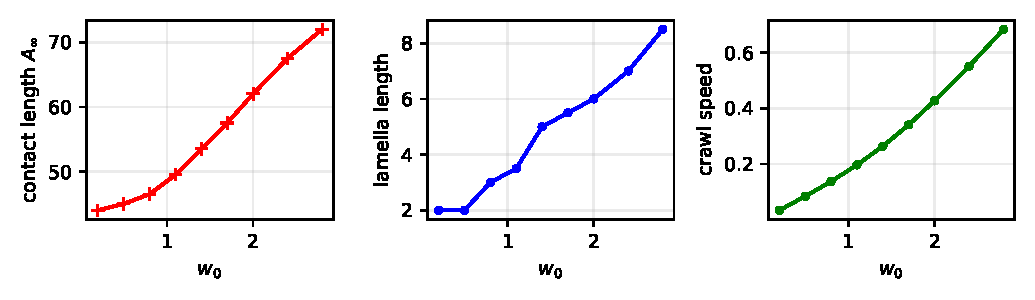
\includegraphics[width=14cm]{figures/fig_v2_transition.pdf}
\caption{{The protrusion transition of Version 2. Steady contact length along the
wall (left), length of the region thinner than $2\lambda$, i.e.\ the extent of the
thin leading layer (centre), and crawl speed (right), against the treadmilling
rate $w_{0}$. The contact length is almost flat below $w_{0}\approx0.8$ and rises
steeply above it, close to the estimate
$M\varepsilon^{2}/\lambda\approx0.75$ obtained by balancing the active push
against interfacial tension at the scale of the protrusion thickness. Each point
continues from the previous steady state.}}
\label{fig:v2transition}
\end{figure}
%%%%%%%%%%%%%%%%%%%%%%%%%%%%%%%%%%%%%%%%%%%%%%%%%%%%%%%%%%%%

\subsection{Version 3: the full model in the plane}
\label{sec:v3}

The cell shapes catalogued in Fig.~2 of Ref.~\cite{Tjhung:2015} are top-view
shapes, so Version 3 works in the $(x,y)$ plane and solves the complete system:
eqs.(\ref{eq:eom}) to (\ref{eq:stresses}) with the spectral Stokes solve of
eq.(\ref{eq:leray}).

Before switching on any activity we verify the passive limit, which exercises the
Stokes solve, the sign of the capillary force and the conservative advection
together. With $w_{0}=\zeta=\beta=0$ and $\mathbf{P}$ frozen at zero, the model
reduces to a viscous drop held by interfacial tension, and all three expected
behaviours are recovered: an initially elliptical drop relaxes to a circle, its
aspect ratio falling from $1.689$ to $1.010$ and its circularity rising from
$0.884$ to $1.002$; the free energy decreases monotonically from $30.488$ to
$28.624$; and the flow decays from $2.16$ to $6.5\times10^{-5}$ while the volume
error stays exactly zero. Had the sign of $-\phi\nabla\mu_\phi$ been wrong the
ellipse would have elongated instead and the run would have diverged. The
calculation is also resolution independent, $N=128$ and $N=160$ agreeing on speed
and aspect ratio to about $1\%$.

Figure~\ref{fig:v3morph} shows three steady states obtained by varying only
$\beta$ and $\zeta$. With strong outward anchoring the polarization locks into a
radial \textbf{aster} with a $+1$ topological defect at the centre. Then
$|\langle\mathbf{P}\rangle|=0$ exactly, the outward arrows cancelling, and since
the cell is transported by $w_{0}\mathbf{P}$ the treadmilling pushes equally in
every direction and nothing moves: the measured speed is of order $10^{-23}$,
zero to machine precision, and the residual flow is negligible at $0.019$ against
$w_{0}=1$. This is the non-motile ``fried egg'' of Ref.~\cite{Tjhung:2015}, and it
reproduces the mechanism identified both there and experimentally
\cite{Yam:2007}, namely that motility requires the actin orientation field to
break symmetry. The other two runs have $|\langle\mathbf{P}\rangle|\approx0.9$ and
crawl at about $0.84$, close to $w_{0}$, as Ref.~\cite{Tjhung:2015} also reports.
At intermediate anchoring the polarization splays, the leading edge broadens, and
the cell becomes a fan elongated \textit{across} its direction of travel with two
trailing wings, which is the \textbf{lamellipodium} morphology of a motile
keratocyte; driving anchoring harder gives more of the same.

%%%%%%%%%%%%%%%%%%%%%%%%%%%%%%%%%%%%%%%%%%%%%%%%%%%%%%%%%%%%
\begin{figure}[ht!]
\centering
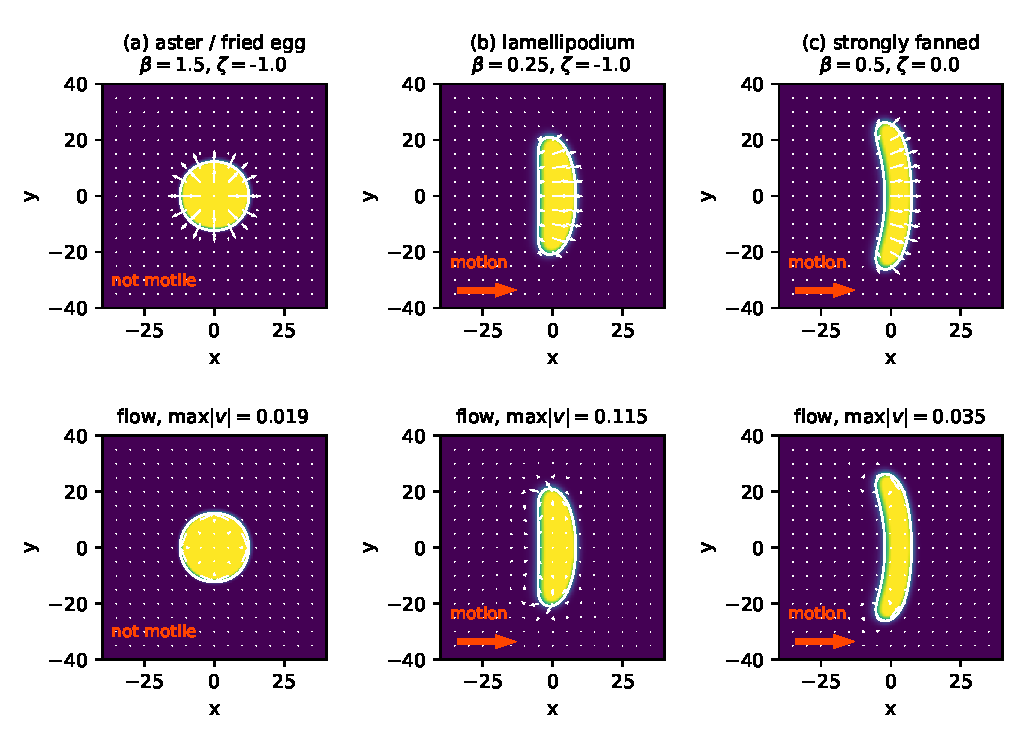
\includegraphics[width=14cm]{figures/fig_v3_morph.pdf}
\caption{{Steady cell morphologies from the full Version 3 model at $w_{0}=1$.
Top row: cell field $\phi$ with the actin polarization $\mathbf{P}$ as white
arrows. Bottom row: the same states with the intracellular flow $\mathbf{v}$. The
orange arrow marks the measured direction of motion, which is essential for
reading the shapes since a cell elongated across its path and one elongated along
it have the same aspect ratio. (a) Strong anchoring produces a radial aster with
$|\langle\mathbf{P}\rangle|=0$ and zero speed to machine precision. (b) Moderate
anchoring gives the lamellipodial fan, aspect ratio $2.91$, speed $0.843$. (c)
Stronger anchoring with no contractility gives a more extreme fan, aspect ratio
$4.35$. Because the $\mathbf{k}=0$ mode of $\mathbf{v}$ is set to zero, the flow
shown is the internal circulation relative to the cell's own drift.}}
\label{fig:v3morph}
\end{figure}
%%%%%%%%%%%%%%%%%%%%%%%%%%%%%%%%%%%%%%%%%%%%%%%%%%%%%%%%%%%%

Two shapes reported in Ref.~\cite{Tjhung:2015} do \textit{not} appear, and in both
cases the reason is geometric rather than numerical. The \textbf{pseudopod}, a
finger pointing along the direction of motion, cannot form: with $\mathbf{P}$
along $\hat{x}$ contractility produces a force $|\zeta|\partial_x\phi$ that
squeezes the cell \textit{along} its polarization axis, so it can only ever widen
the cell across its path. In Ref.~\cite{Tjhung:2015} the pseudopod is set by the
vertical confinement of treadmilling, eq.(\ref{eq:wz}), and a top view has no $z$;
Version 2 captures exactly that structure instead, so between the two the
mechanism is covered. The \textbf{phagocytic cup} does not appear either:
increasing $\beta$ at $\zeta=0$ gives fan, then a more extreme fan, then cells
that stop crawling straight and begin to turn, and finally the non-motile aster,
with no indented leading edge anywhere along the sequence. In
Ref.~\cite{Tjhung:2015} this shape is explicitly three-dimensional.

The most useful result of Version 3 is a control experiment that is not in
Ref.~\cite{Tjhung:2015}. The model contains two candidate mechanisms for
deforming the cell: anchoring, which splays $\mathbf{P}$ and thereby makes the
treadmilling transport $w_{0}\mathbf{P}$ non-uniform, and which needs no flow at
all; and the flow itself, acting through the active and elastic stresses.
Switching each on and off independently gives the $2\times2$ of
figure~\ref{fig:v3decomp}. With neither, the cell is a translating disc of aspect
ratio $1.07$, which is Version 1. The flow alone \textit{does} deform it,
$1.07\rightarrow1.61$, and is the only mechanism available when $\beta=0$.
Anchoring alone is much stronger, $1.07\rightarrow2.85$. But adding the flow on
top of anchoring buys almost nothing, $2.85\rightarrow2.92$, about $2\%$: the two
mechanisms are strongly sub-additive. The reason the increment is so small is
that the flow contains competing pieces, the contractile part elongating the
cell and the passive capillary and elastic part rounding it off; removing
contractility at $\beta=0.25$ in fact \textit{lowers} the aspect ratio to $2.64$,
below the flow-free value. Flow alignment does essentially nothing, $2.94$ against
$2.92$. The crawl speed is $0.80$ to $0.85$ in every case, because it is set by
$w_{0}\langle\mathbf{P}\rangle$.

%%%%%%%%%%%%%%%%%%%%%%%%%%%%%%%%%%%%%%%%%%%%%%%%%%%%%%%%%%%%
\begin{figure}[ht!]
\centering
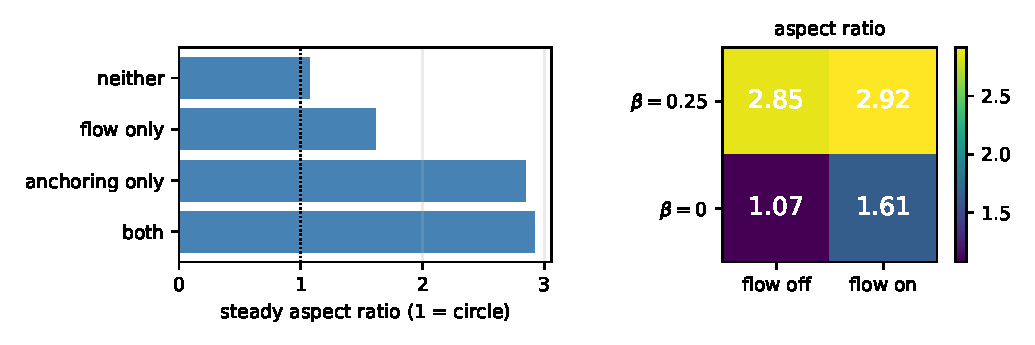
\includegraphics[width=14cm]{figures/fig_v3_decomp.pdf}
\caption{{Which ingredient sets the cell shape in the plane. Steady aspect ratio
for the four combinations of anchoring on/off and hydrodynamic flow on/off, at
otherwise identical parameters ($w_{0}=1$, $\zeta=-1$). Anchoring alone takes the
aspect ratio from $1.07$ to $2.85$; the flow alone takes it to $1.61$; both
together give $2.92$, only $2\%$ above anchoring alone. In this geometry the cell
shape is therefore predominantly anchoring-driven rather than hydrodynamic, which
is what justifies the approximation made in Version 4.}}
\label{fig:v3decomp}
\end{figure}
%%%%%%%%%%%%%%%%%%%%%%%%%%%%%%%%%%%%%%%%%%%%%%%%%%%%%%%%%%%%

Finally, varying the substrate friction $\xi$ over a $32$-fold range gives three
clean observations. The internal flow is screened, falling by an order of
magnitude and steepening towards $1/\xi$ at strong adhesion, as
eq.(\ref{eq:leray}) predicts once $\xi\gg\eta k^{2}$. The crawl speed barely
moves, from $0.829$ to $0.845$, which follows directly from the structure of the
model: the cell is transported by $\mathbf{u}=\mathbf{v}+w_{0}\mathbf{P}$, the
mean of $\mathbf{v}$ vanishes, and so the speed is
$w_{0}\langle\mathbf{P}\rangle$ whatever the friction. And the shape depends on
adhesion monotonically and \textit{saturates}: the aspect ratio falls from $3.93$
to $2.81$ and then flattens, onto the independently measured flow-free value of
$2.85$. That agreement is a free consistency check on the Stokes solve, and it is
also the observation that motivates Version 4.

The flat speed is worth flagging as a genuine \textit{disagreement} with
Ref.~\cite{Leoni:2017}, whose central result is that migration speed is strongly
and non-monotonically dependent on adhesion. The two models put the motor in
different places. Here, propulsion comes from treadmilling and adhesion only
damps the flow that this generates. In Ref.~\cite{Leoni:2017}, propulsion comes
from traction against the substrate, and the net displacement per cycle exists
\textit{only} because the bonds are mechanosensitive, so that the drag differs
between protrusion and retraction; their result is proportional to the stress
sensitivity and vanishes without it. Their mechanism is therefore invisible to a
model with a constant $\xi$, and capturing it would require both a load-dependent
friction and a cycle in the activity for that friction to rectify.

\subsection{Version 4: a tractable model}
\label{sec:v4}

Version 3 answers what the full model does, but its Stokes solve makes it too
expensive to extend to many cells: eq.(\ref{eq:stokes}) is elliptic, so
$\mathbf{v}$ at each point depends on $\mathbf{f}$ everywhere and cannot be
evaluated pointwise. The two dissipative terms in eq.(\ref{eq:stokes}) enter as
$\eta k^{2}$ and $\xi$, however, so their ratio is
\begin{equation}\label{eq:ratio}
\frac{\eta k^{2}}{\xi}\sim\frac{\eta}{\xi R^{2}}\approx 0.006
\end{equation}
for a cell of radius $R\approx13$ with $\eta=\xi=1$: substrate friction, not
viscosity, is what balances the active forces. Dropping the viscous term, and
with it the incompressibility constraint whose only role was to determine the
pressure, leaves
\begin{equation}\label{eq:darcy}
\xi\mathbf{v}=\mathbf{f}
\qquad\Longrightarrow\qquad
\mathbf{v}=\mathbf{f}/\xi,
\end{equation}
which is \textit{local and algebraic}. This friction-dominated, or Darcy, limit is
the standard basis for computationally cheap two-dimensional crawling-cell models
\cite{Ziebert:2013}. It is a controlled approximation rather than a guess, and
Version 3 has already measured the approach to it: the adhesion sweep of
Sec.~\ref{sec:v3} showed the flow falling off as $1/\xi$ and the shape saturating
onto its own flow-free limit as adhesion was increased. Through
eq.(\ref{eq:darcy}) the capillary part of $\mathbf{f}$ would contribute a
relaxation of the same character as the $-M\mu_\phi$ term already present, so it
is absorbed into $M$ and only the active part
$\mathbf{v}=-(\zeta/\xi)\nabla\cdot(\phi\mathbf{P}\mathbf{P})$ is retained.
Vorticity and flow alignment are dropped as well, Version 3 having measured them
to change the steady shape by well under $1\%$. Parameters are listed in
table~\ref{tab:v4param}.

%%%%%%%%%%%%%%%%%%%%%%%%%%%%%%%%%%%%%%%%%%%%%%%%%%%%%%%%%%%%
\begin{table} [ht!]
\begin{center}
\begin{tabular}{ |c|c|c|c| }
 \hline
 Quantity & Symbol & Value & Role \\
 \hline
 grid, box size & $N$, $L$ & $128^{2}$, $80$ & $dx=0.625$, interface spans $3.4$ cells\\
 \hline
 initial radius & $R_{0}$ & $13$ & cell size \\
 \hline
 interface width & $\varepsilon$ & $1.5$ & sets interfacial tension with $M$ \\
 \hline
 relaxation rate & $M$ & $1$ & interfacial relaxation \\
 \hline
 polar bulk strength & $\alpha$ & $0.5$ & gives $|\mathbf{P}|=1$ inside \\
 \hline
 Frank constant & $\kappa$ & $1$ & polarization elasticity \\
 \hline
 rotational viscosity & $\Gamma$ & $1$ & polarization relaxation rate \\
 \hline
 treadmilling rate & $w_{0}$ & $1$ & sets the crawl speed \\
 \hline
 active stress & $\zeta$ & $-0.25$ & contractile; recalibrated, see text \\
 \hline
 anchoring & $\beta$ & $0.15$ & sets the shape \\
 \hline
 substrate friction & $\xi$ & $1$ & adhesion strength \\
 \hline
 area stiffness & $k_{A}$ & $5$ & soft volume constraint, eq.(\ref{eq:soft}) \\
 \hline
 time step & $dt$ & $0.02$ & $dt<dx^{2}/(4M\varepsilon^{2})=0.043$ \\
 \hline
\end{tabular}
\end{center}
\caption{Parameters used for the Version 4 results, in simulation units.}
\label{tab:v4param}
\end{table}
%%%%%%%%%%%%%%%%%%%%%%%%%%%%%%%%%%%%%%%%%%%%%%%%%%%%%%%%%%%%

The first question to settle is simply whether the cell moves, so
figure~\ref{fig:v4montage} answers it in the plainest way available, by drawing
the cell outline in the \textit{laboratory} frame at successive times. It travels
$239.9$ length units in $299$ time units at a steady speed of $0.801$ against
$w_{0}=1$, in a straight line, while turning from a disc into a fan. The same run
is shown cell-centred with the polarization field in
figure~\ref{fig:v4snapshots}, and the corresponding time series in
figure~\ref{fig:v4diag}: the trajectory is linear, the speed plateaus almost
immediately, and the aspect ratio saturates by $t\approx150$, so this is a genuine
steady state rather than a transient. The whole run takes $16$ seconds.

%%%%%%%%%%%%%%%%%%%%%%%%%%%%%%%%%%%%%%%%%%%%%%%%%%%%%%%%%%%%
\begin{figure}[ht!]
\centering
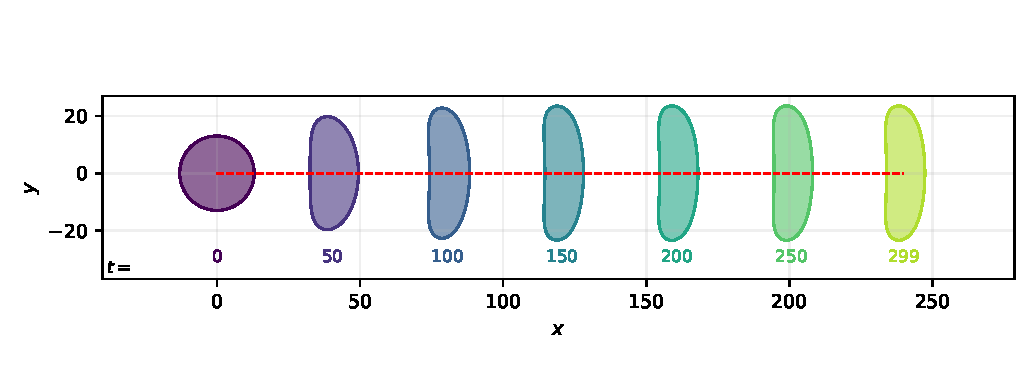
\includegraphics[width=14cm]{figures/fig_v4_montage.pdf}
\caption{{Version 4: the cell in the laboratory frame at successive times, the
label under each outline giving $t$. Filled regions show $\phi>1/2$ and the
dashed red line is the centre-of-mass trajectory. The cell travels $239.9$ length
units in $299$ time units at a steady speed of $0.801$, while developing a fan
shape from an initially circular one. This figure is the direct answer to whether
the model produces a crawling cell.}}
\label{fig:v4montage}
\end{figure}
%%%%%%%%%%%%%%%%%%%%%%%%%%%%%%%%%%%%%%%%%%%%%%%%%%%%%%%%%%%%

%%%%%%%%%%%%%%%%%%%%%%%%%%%%%%%%%%%%%%%%%%%%%%%%%%%%%%%%%%%%
\begin{figure}[ht!]
\centering
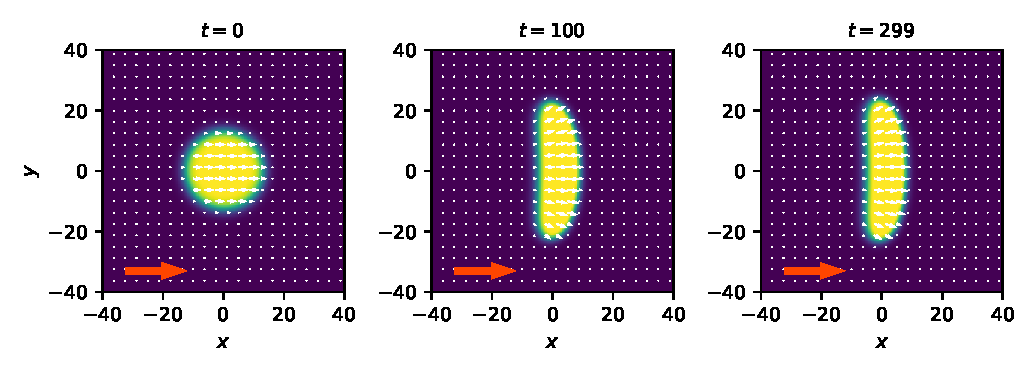
\includegraphics[width=14cm]{figures/fig_v4_snapshots.pdf}
\caption{{The same Version 4 run as figure~\ref{fig:v4montage}, now
cell-centred, showing the cell field $\phi$ with the actin polarization
$\mathbf{P}$ as white arrows at three times. The orange arrow marks the direction
of motion. The polarization splays near the boundary because of the anchoring
term in eq.(\ref{eq:F}), which is what makes the treadmilling transport
non-uniform and so deforms the initially circular cell into a fan.}}
\label{fig:v4snapshots}
\end{figure}
%%%%%%%%%%%%%%%%%%%%%%%%%%%%%%%%%%%%%%%%%%%%%%%%%%%%%%%%%%%%

%%%%%%%%%%%%%%%%%%%%%%%%%%%%%%%%%%%%%%%%%%%%%%%%%%%%%%%%%%%%
\begin{figure}[ht!]
\centering
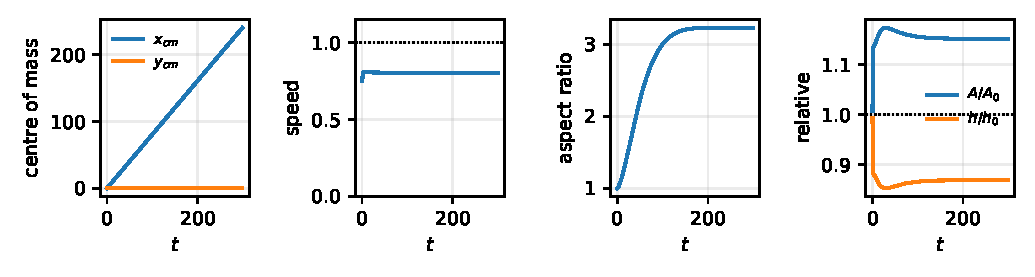
\includegraphics[width=14cm]{figures/fig_v4_diagnostics.pdf}
\caption{{Version 4 diagnostics against time. From left to right: centre of mass,
showing linear motion along $x$ with no drift in $y$; crawl speed, which
plateaus at $0.801$ (the dotted line marks $w_{0}=1$); aspect ratio, saturating by
$t\approx150$; and the projected area $A/A_{0}$ together with the implied
thickness $h/h_{0}=A_{0}/A$ from eq.(\ref{eq:volume}). The last panel is the
point of Sec.~\ref{subsec:volume} made concrete: the cell spreads by $15\%$ and
thins by the same factor at constant volume, which a rigid-area model forbids.}}
\label{fig:v4diag}
\end{figure}
%%%%%%%%%%%%%%%%%%%%%%%%%%%%%%%%%%%%%%%%%%%%%%%%%%%%%%%%%%%%

The effect of the volume treatment is examined in figure~\ref{fig:v4area} by
scanning the stiffness $k_{A}$ of eq.(\ref{eq:soft}), and the outcome is more
nuanced than expected. Relaxing the constraint does free the motion, confirming
the direction of the expectation, but the effect on \textit{speed} is small: from
rigid area to $k_{A}=2$ the crawl speed rises only from $0.7981$ to $0.8040$,
under one per cent. Where the constraint matters is the \textit{shape}: over the
same range the steady aspect ratio moves from $2.86$ to $3.85$, a change of
$35\%$, because a cell permitted to spread fans out further. The soft constraint
also behaves properly as a dynamical variable, the area rising, settling and then
being held rather than drifting.

Removing the constraint altogether, on the other hand, does not work at all. With
$k_{A}=0$ the cell inflates by a factor of $14.2$ until it fills the periodic box,
its thickness falls to $0.07$, its aspect ratio collapses back to $1$ and it
ceases to be a crawling cell; once it touches the boundary the position
measurement is meaningless as well, so no speed is quoted. The cause is
thermodynamic and can be read off eq.(\ref{eq:mu_h}): the $-\alpha|\mathbf{P}|^{2}$
term makes the polarised interior cheaper than the exterior, so the cell grows
until something stops it. Ref.~\cite{Tjhung:2015} never encounters this because
its Cahn--Hilliard dynamics conserves area identically. The conclusion is that the
volume constraint should be \textit{soft rather than absent}.

%%%%%%%%%%%%%%%%%%%%%%%%%%%%%%%%%%%%%%%%%%%%%%%%%%%%%%%%%%%%
\begin{figure}[ht!]
\centering
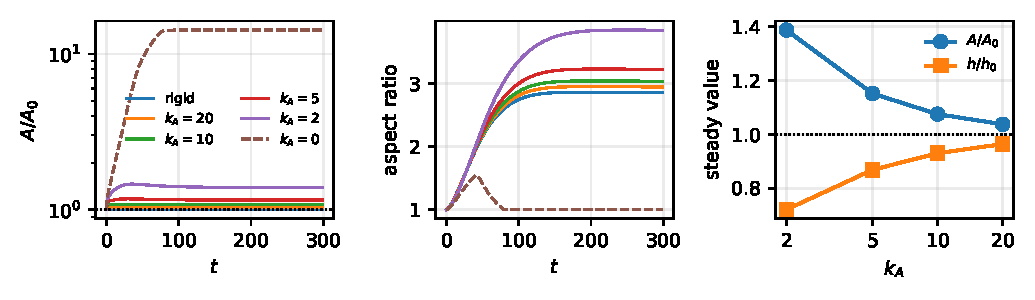
\includegraphics[width=14cm]{figures/fig_v4_area.pdf}
\caption{{Effect of the volume treatment in Version 4. Left: projected area
against time for stiffnesses $k_{A}$ of eq.(\ref{eq:soft}), including the rigid
limit of eq.(\ref{eq:rigid}); note the logarithmic scale. Centre: the
corresponding aspect ratios. Right: steady area and implied thickness against
$k_{A}$. A soft constraint lets the cell spread and thin and then hold that
state, whereas with no constraint at all ($k_{A}=0$, dashed) the cell inflates
$14.2$-fold until it fills the box and stops crawling.}}
\label{fig:v4area}
\end{figure}
%%%%%%%%%%%%%%%%%%%%%%%%%%%%%%%%%%%%%%%%%%%%%%%%%%%%%%%%%%%%

Two checks establish that the cheap model has not quietly become a different one.
The cost, first: table~\ref{tab:speed} shows that removing the Fourier transforms
reduces the time per step from $2.70$ to $1.10$ ms, and that the largest stable
time step grows threefold, giving roughly a fivefold overall saving at the
default $dt=0.02$ and sevenfold at $dt=0.03$. The step size is verified by
convergence: over $dt=0.01$, $0.02$ and $0.03$ the steady aspect ratio changes by
$0.6\%$ and the speed agrees to four significant figures.

Second, and more importantly, Version 4 can be compared with Version 3 in the
limit where the two \textit{should} coincide. Switching the flow off and holding
the area rigid reduces Version 4 to exactly the ``anchoring only'' control run of
figure~\ref{fig:v3decomp}. Version 3 measured a steady aspect ratio of $2.850$
and a speed of $0.846$ there; Version 4 gives $2.855$ and $0.845$, an agreement of
$0.2\%$. The two codes were written independently and share no solver machinery,
so this is a meaningful check rather than a tautology.

One difference does \textit{not} vanish and must be stated. With the active flow
switched back on, the friction-dominated velocity deforms the cell considerably
more than the incompressible Stokes flow did at the same $\zeta$: Version 3 gives
an aspect ratio of $2.92$ at $\zeta=-1$, whereas Version 4 reaches about $5.9$.
The missing pressure is the reason, incompressibility having resisted the
deformation in Version 3 with nothing to replace it here. The activity parameter
is therefore roughly an order of magnitude more potent in Version 4, which is why
table~\ref{tab:v4param} uses $\zeta=-0.25$ rather than $-1$. The shapes belong to
the same family; only the calibration of $\zeta$ changes. Consistently with
Version 3, anchoring remains the controlling shape parameter: $\beta=0$, $0.05$,
$0.15$ and $0.25$ give steady aspect ratios of $1.37$, $2.12$, $3.23$ and $4.31$.

%%%%%%%%%%%%%%%%%%%%%%%%%%%%%%%%%%%%%%%%%%%%%%%%%%%%%%%%%%%%
\begin{table} [ht!]
\begin{center}
\begin{tabular}{ |c|c|c| }
 \hline
 Quantity & Version 3 & Version 4 \\
 \hline
 force balance & incompressible Stokes, spectral & friction dominated, local \\
 \hline
 transforms per step & 4 & 0 \\
 \hline
 time per step at $128^{2}$ & $2.70$ ms & $1.10$ ms \\
 \hline
 largest stable $dt$ & $0.01$ & $0.03$ \\
 \hline
 one run to steady state & $\approx60$ s & $16$ s \\
 \hline
 overall saving & --- & $\approx5\times$ at $dt=0.02$ \\
 \hline
\end{tabular}
\end{center}
\caption{Cost of the full and reduced force balances, measured on the same
$128^{2}$ grid. The saving in wall-clock time matters, but the structural point
matters more: in Version 4 every operation is a local stencil, so the cost is
linear in the number of grid points with no global coupling, which is the
property an elliptic solve destroys and the property that makes many cells
affordable.}
\label{tab:speed}
\end{table}
%%%%%%%%%%%%%%%%%%%%%%%%%%%%%%%%%%%%%%%%%%%%%%%%%%%%%%%%%%%%

%%%%%%%%%%%%%%%%%%%%%%%%%%%%%%%%%%%%%%%%%%%%%%%%%%%%%%%%%%%%
%%%%%%%%%%%%%%%%%%%%%%%%%%%%%%%%%%%%%%%%%%%%%%%%%%%%%%%%%%%%
\section{Conclusions}
\label{sec:Conclusion}
%%%%%%%%%%%%%%%%%%%%%%%%%%%%%%%%%%%%%%%%%%%%%%%%%%%%%%%%%%%%
%%%%%%%%%%%%%%%%%%%%%%%%%%%%%%%%%%%%%%%%%%%%%%%%%%%%%%%%%%%%
Based on the discussion presented in section \ref{sec:results}, the position
reached is as follows.

\begin{itemize}
\item A phase-field model of a crawling cell has been implemented in four stages
and verified at each. Volume is now conserved to machine precision where it
should be, against a $4.5\%$ drift in the starting version, and the passive limit
of the full model behaves correctly, an elliptical drop relaxing to a circle with
monotonically decreasing free energy and a flow that dies away.

\item Confining treadmilling to a layer of thickness $\lambda$ at the substrate
produces a thin leading protrusion and steady crawling, together with a
protrusion transition in $w_{0}$ whose threshold agrees with the estimate obtained
by balancing the active push against interfacial tension at the scale $\lambda$.

\item The full model in the plane reproduces the non-motile actin aster, in which
$|\langle\mathbf{P}\rangle|=0$ and the speed vanishes to machine precision, and
the lamellipodial fan of a motile keratocyte, at speeds close to $w_{0}$. It does
not reproduce the pseudopod or the phagocytic cup, and in both cases the reason is
that these are structures of the geometry we have projected out rather than a
defect of the implementation.

\item Isolating ingredients shows that in the plane the cell shape is
predominantly set by anchoring-induced splay of the polarization, which requires
no flow: anchoring alone raises the aspect ratio from $1.07$ to $2.85$, whereas
adding the full hydrodynamics on top of it contributes a further $2\%$. This is
not what one would guess from the literature and it is the key result guiding the
rest of the project.

\item Acting on that, the elliptic Stokes solve has been replaced by its
friction-dominated limit, justified both by the parameter estimate
$\eta/\xi R^{2}\approx0.006$ and by the observed saturation of the full model onto
its own flow-free limit at strong adhesion. The reduced model is about five times
faster, agrees with the full one to $0.2\%$ where they coincide, and is local in
structure.

\item Conserving cell volume rather than projected area lets the cell spread by
$15\%$ and thin by the same factor while crawling. The effect on speed is under
one per cent, but the effect on shape is $35\%$. Removing the constraint entirely
is not viable: the cell then inflates $14$-fold and stops crawling.
\end{itemize}

%%%%%%%%%%%%%%%%%%%%%%%%%%%%%%%%%%%%%%%%%%%%%%%%%%

%%%%%%%%%%%%%%%%%%%%%%%%%%%%%%%%%%%%%%%%%%%%%%%%%%%%%%%%%%%%
%%%%%%%%%%%%%%%%%%%%%%%%%%%%%%%%%%%%%%%%%%%%%%%%%%%%%%%%%%%%
\section{Future scope}
\label{sec:scope}
%%%%%%%%%%%%%%%%%%%%%%%%%%%%%%%%%%%%%%%%%%%%%%%%%%%%%%%%%%%%
%%%%%%%%%%%%%%%%%%%%%%%%%%%%%%%%%%%%%%%%%%%%%%%%%%%%%%%%%%%%
The work plan for the remainder of the project is to move from one cell to many,
which is what the reduced model of Sec.~\ref{sec:v4} was constructed for. The
steps, in order, are:

\begin{enumerate}
\item \textbf{Two interacting cells.} Introduce one phase field $\phi_i$ per cell,
each with its own polarization $\mathbf{P}_i$, so that cells remain
distinguishable rather than merging, and add a repulsive overlap term
$\varepsilon_{rep}\sum_{i\neq j}\phi_i^{2}\phi_j^{2}$ to eq.(\ref{eq:F}) to
generate contact forces. The soft volume constraint of eq.(\ref{eq:soft}) already
extends naturally, one target area $A_{0,i}$ per cell. Re-centring must be
replaced by a fixed laboratory frame with a domain large enough for the cells to
move in, since separate cells cannot all be centred. None of this requires a
solver, and the cost grows linearly in the number of cells, with the overlap term
growing as the number of neighbouring pairs, which stays cheap if a cell list is
used.

\item \textbf{Collision phenomenology.} With two cells available, study head-on
and glancing collisions and measure whether the model reproduces contact
inhibition of locomotion, in which colliding cells stop and repolarise away from
one another. This is a genuine prediction to test rather than an input.

\item \textbf{Spontaneous polarity.} At present the direction of motion is
inherited from the initial condition, either uniform or radial. Replacing this by
a polarity module with a conserved total, of the kind used to describe
spontaneous symmetry breaking in cell fragments \cite{Verkhovsky:1999,Yam:2007},
would let each cell choose its own direction and would make collision outcomes
meaningful.

\item \textbf{Mechanosensitive adhesion.} Section \ref{sec:v3} showed that with a
constant $\xi$ the crawl speed is essentially independent of adhesion, in contrast
to Ref.~\cite{Leoni:2017}. Making the friction depend on local traction, together
with a cycle in the activity for it to rectify, would test that prediction inside
a continuum model and is the natural way to connect the two descriptions.

\item \textbf{Small collectives.} Finally, tens of cells, to look for the
collective effects that motivate the whole exercise: jamming at high density, and
alignment of motility with neighbours of the kind implicated in wound healing.
\end{enumerate}
%%%%%%%%%%%%%%%%%%%%%%%%%%%%%%%%%%%%%%%%%%%%%%%%%%


\section*{Acknowledgements}
%%%%%%%%%%%%%%%%%%%%%%%%%%%%%%%%%%%%%%%%%%%%%%%%%%%%%%%%%%%%
% FILLME: replace the adviser's name, and add anything else appropriate.
The author would like to thank Prof.\ Firstname Lastname for suggesting this
problem, for guidance on the choice of model, and in particular for pointing out
that the projected area of a crawling cell should not be held fixed and that an
alternative to solving the Stokes equation would be needed before the work could
be extended to many cells. Both suggestions shaped
Sec.~\ref{sec:v4} of this report.
%%%%%%%%%%%%%%%%%%%%%%%%%%%%%%%%%%%%%%%%%%%%%%%%%%%%

%%%%%%%%%%%%%%%%%%%%%%%%%%%%%%%%%%%%%%%%%%%%%%%%%%%%%%%%%%%%
%\appendix
%%%%%%%%%%%%%%%%%%%%%%%%%%%%%%%%%%%%%%%%%%%%%%%%%%%%%%%%%%%%

%%%%%%%%%%%%%%%%%%%%%%%%%%%%%%%%%%%%%%%%%%%%%%%%%%%%%%%%%%%%
%References
\begin{thebibliography}{99}
%%%%%%%%%%%%%%%%%%%%%%%%%%%%%%%%%%%%%%%%%%%%%%%%%%%%%%%%%%%%
\bibitem{Bray:2000}
  D.~Bray,
  ``Cell Movements: From Molecules to Motility,'' 2nd edition,
  Garland Science (2000) 386p,
  ISBN: 9780815332824.
  %%%%%%%%%
\bibitem{Verkhovsky:1999}
  A.~B.~Verkhovsky, T.~M.~Svitkina and G.~G.~Borisy,
  ``Self-polarization and directional motility of cytoplasm,''
  Curr.\ Biol.\  {\bf 9}, no. 1, 11 (1999).
%%%%%%%%%
\bibitem{Keren:2008}
  K.~Keren, Z.~Pincus, G.~M.~Allen, E.~L.~Barnhart, G.~Marriott,
  A.~Mogilner and J.~A.~Theriot,
  ``Mechanism of shape determination in motile cells,''
  Nature {\bf 453}, 475 (2008).
%%%%%%%%%
\bibitem{Barnhart:2011}
  E.~L.~Barnhart, K.~C.~Lee, K.~Keren, A.~Mogilner and J.~A.~Theriot,
  ``An adhesion-dependent switch between mechanisms that determine motile cell
  shape,''
  PLoS Biol.\  {\bf 9}, no. 5, e1001059 (2011).
%%%%%%%%%
\bibitem{Tjhung:2015}
  E.~Tjhung, A.~Tiribocchi, D.~Marenduzzo and M.~E.~Cates,
  ``A minimal physical model captures the shapes of crawling cells,''
  Nat.\ Commun.\  {\bf 6}, 5420 (2015).
%%%%%%%%%
\bibitem{Tjhung:2012}
  E.~Tjhung, D.~Marenduzzo and M.~E.~Cates,
  ``Spontaneous symmetry breaking in active droplets provides a generic route to
  motility,''
  Proc.\ Natl.\ Acad.\ Sci.\ USA {\bf 109}, no. 31, 12381 (2012).
%%%%%%%%%
\bibitem{Leoni:2017}
  M.~Leoni and P.~Sens,
  ``Model of cell crawling controlled by mechanosensitive adhesion,''
  Phys.\ Rev.\ Lett.\  {\bf 118}, no. 22, 228101 (2017).
%%%%%%%%%
\bibitem{Ziebert:2013}
  F.~Ziebert and I.~S.~Aranson,
  ``Effects of adhesion dynamics and substrate compliance on the shape and
  motility of crawling cells,''
  PLoS ONE {\bf 8}, no. 5, e64511 (2013).
%%%%%%%%%
\bibitem{deGennes:1993}
  P.~G.~de Gennes and J.~Prost,
  ``The Physics of Liquid Crystals,'' 2nd edition,
  Clarendon Press, Oxford (1993) 597p,
  ISBN: 9780198517856.
%%%%%%%%%
\bibitem{Rubinstein:1992}
  J.~Rubinstein and P.~Sternberg,
  ``Nonlocal reaction-diffusion equations and nucleation,''
  IMA J.\ Appl.\ Math.\  {\bf 48}, no. 3, 249 (1992).
%%%%%%%%%
\bibitem{Yam:2007}
  P.~T.~Yam, C.~A.~Wilson, L.~Ji, B.~Hebert, E.~L.~Barnhart, N.~A.~Dye,
  P.~W.~Wiseman, G.~Danuser and J.~A.~Theriot,
  ``Actin-myosin network reorganization breaks symmetry at the cell rear to
  spontaneously initiate polarized cell motility,''
  J.\ Cell Biol.\  {\bf 178}, no. 7, 1207 (2007).
\end{thebibliography}
%%%%%%%%%%%%%%%%%%%%%%%%%%%%%%%%%%%%%%%%%%%%%%%%%%%%%%%%%%%%
\end{document}
